\chapter{Software}
This chapter contain the software that is used for developing and testing the autonomous landing system for uav. 

The software that is mainly used in the uav system is based on a open-source software toolchain developed by the Underwater System and Technology Laboratory (LSTS). The toolchain supports air and ocean vehicle systems. The different components in the toolchain is IMC, DUNE, NEPTUS and Glued, which will be presented in later in this chapter. 

The rtkgps solution in the system is calculated in the open-source software RtkLib \citep{takasu2009development}. The desceription of the program is given in section \ref{s:Rtklib}.

The low level control system in the uav is controlled by Ardupilot, which is a 
\section{IMC}
IMC \citep{martins2009imc} is the communication protocol that is used for all communication within and between DUNE and Neptus. The message protocol is oriented around the message. All messages is pre-set  The entire complete protocol is defined in one XML document. 
\section{Dune}
Dune is a open-source software framework in which each Dune tasks are run in a separated threads. Each task communicate with an other with IMC messages. 
\section{Neptus}
\section{Glued}

\section{RTKLIB}\label{ss:Rtklib}
\acrfull{rtklib}\citep{takasu2009development} is a open source program package for standard and precise positioning with \gls{gnss} developed by T. Takasu. \gls{rtklib} can be configured to apply \gls{rtk-gps}, such that raw \gls{gnss} data is used estimate the relative position of the rover with respect to the base station in real time. Figure \ref{figure:RTKLIB_STRUCTURE} shows how \gls{rtklib} can be used in a \gls{rtk-gps} mode. The two main modules here is str2str and rtkrcv. Both will be explained more closely in the following sections. The version of \gls{rtklib} used in this thesis is \gls{rtklib}2.4.2 \citep{Rtklib242}.
\begin{figure}[H]
	\centering
		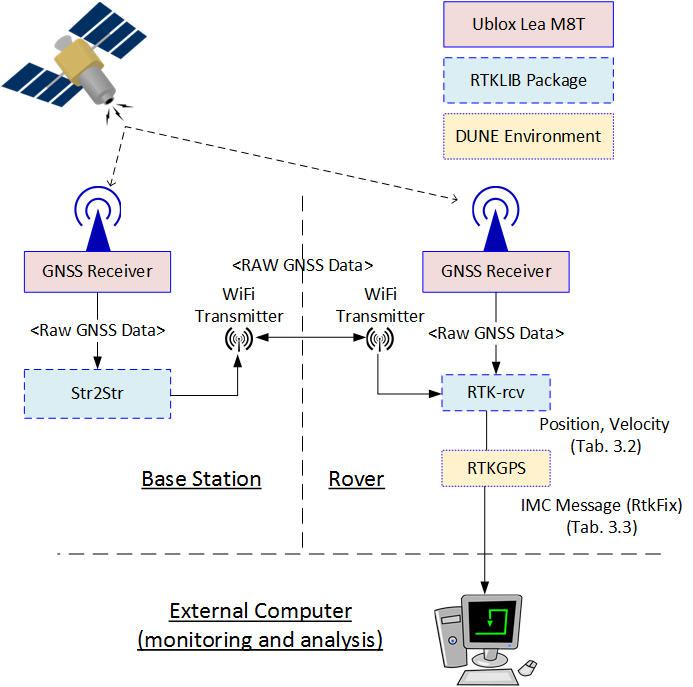
\includegraphics[width=1\textwidth]{figs/RTKLIB.png}
		\caption{The communication structure of \gls{rtklib}}
		\label{figure:RTKLIB_STRUCTURE}
\end{figure}
\subsection{Rtkrcv}
As part of the \gls{rtklib} Rtkrcv is  used to calculate the position of the rover in real time. Rtkrcv can be configured to have two output streams. It's desired in a automatic landing system to have a velocity estimate. However this is not provided in the newest version of \gls{rtklib}, and therefore a altered version of \gls{rtklib} is used in the navigation system where the velocity is part of the output data. The position output is in \gls{enu} format and the full output structure is presented in table \ref{Tb:RtklibOutput}
\begin{table}[H]
\begin{center}
    \begin{tabular}{ | l | l |}
    \hline
    \textbf{Header} & \textbf{Content} \\ \hline
     1 Time & The epoch time of the solution indicate the true receiver\\& signal reception time. Can have the following format:\\&\\& yyyy/mm/dd HH:MM:SS.SSS:\\& Calender time in GPST, UTC or JST.\\&\\&
     
     WWWW SSSSSSS.SSS:\\&
     GPS week and TOW in seconds  \\ \hline
     2 Receiver Position & The rover receive antenna position \\ \hline
     3 Quality flag (Q) & The flag which indicates the solution quality.\\& 1:Fixed\\& 2:Float\\& 5:Single \\ \hline
     4 Number of valid satellites (ns) & The number of valid satellites for solution estimation. \\ \hline
     5 Standard deviation & The estimated standard deviation of the\\& solution assuming a priori error model and error\\& parameters by the positioning options \\ \hline
     6 Age of differential & The time difference between the observation data epochs\\& of the rover receiver and base station in second. \\ \hline
     7 Ratio factor & The ratio factor of "ratio-test" for standard integer\\& ambiguity validation strategy \\ \hline
     8 Receiver velocity & The velocity of the rover. Given only when output is\\& in enu format \\ \hline
    \end{tabular}
\end{center}
\caption{Rtklib output solution format }
\label{Tb:RtklibOutput}
\end{table}
\subsection{Str2str}
Str2str is used as a base station program that can receive raw \gls{gnss} data and further export data over tcp, set-up by str2str. Str2str sends out Radio Technical Commission for Maritime Service 3 (RMTC3) formatted messages, however it can be configured to send whatever comes in as input. The communication between str2str and rtkrcv is shown i figure \ref{figure:RTKLIB_STRUCTURE}
\section{Ardopilot}
\section{JSBsim}